\documentclass{oblivoir}
\usepackage{amsmath,amssymb,amsthm,kotex,paralist,kswrapfig}

\usepackage[skipabove=10pt,innertopmargin=10pt]{mdframed}

\usepackage{tabto,pifont}
\TabPositions{0.2\textwidth,0.4\textwidth,0.6\textwidth,0.8\textwidth}
\newcommand\tabb[5]{\par\bigskip\noindent
\ding{172}\:{\ensuremath{#1}}
\tab\ding{173}\:\:{\ensuremath{#2}}
\tab\ding{174}\:\:{\ensuremath{#3}}
\tab\ding{175}\:\:{\ensuremath{#4}}
\tab\ding{176}\:\:{\ensuremath{#5}}}

\usepackage{enumitem}
\setlist[enumerate]{label=(\arabic*)}

\newcounter{num}
\newcommand{\defi}[1]
{\noindent\refstepcounter{num}\textbf{정의 \arabic{num}) #1}\par\noindent}
\newcommand{\theo}[1]
{\noindent\refstepcounter{num}\textbf{정리 \arabic{num}) #1}\par\noindent}
\newcommand{\exam}[1]
{\bigskip\bigskip\noindent\refstepcounter{num}\textbf{예시 \arabic{num}) #1}\par\noindent}
\newcommand{\prob}[1]
{\bigskip\bigskip\noindent\refstepcounter{num}\textbf{문제 \arabic{num}) #1}\par\noindent}
\newcommand{\proo}
{\bigskip\textsf{증명)}\par}

\newcommand{\ans}{
{\par
\raggedleft\textbf{답 : (\qquad\qquad\qquad\qquad\qquad\qquad)}
\par}\bigskip\bigskip}

\newcommand{\pb}[1]%\Phantom + fBox
{\fbox{\phantom{\ensuremath{#1}}}}

\newcommand\ba{\,|\,}

\newcommand\an[1]{\par\bigskip\noindent\textbf{문제 #1)}\\}

\let\oldsection\section
\renewcommand\section{\clearpage\oldsection}

\renewcommand{\arraystretch}{1.5}

\let\emph\textsf
%%%%
\begin{document}

\title{윤영 : 08 명제(1)}
\author{}
\date{\today}
\maketitle
\tableofcontents
\newpage

%%

%%
\section{명제의 뜻}

%
\exam{}
다음 중 참인 것을 고르시오.
\begin{enumerate}
\item
독도는 대한민국의 영토이다,
\item
달은 지구 주위를 공전한다,
\item
제주도는 큰 섬이다.
\item
1+2>4
\end{enumerate}
위의 예에서 (1)과 (2)는 참인 문장이고 (4)는 거짓인 문장이다.
(3)의 경우에는 참이라고 할 수도 없고 거짓이라고 할 수도 없다.
`큰 섬'의 기준이 명확하지 않기 때문이다.
\begin{mdframed}

%
\defi{명제}
(1), (2), (4)처럼 그 내용이 참인지 거짓인지를 명확하게 판별할 수 있는 문장이나 식을 \emph{명제}라고 한다.
(1), (2)는 참인 명제이고 (4)는 거짓인 명제이다.
\end{mdframed}

%
\prob{}
다음 중 명제인 것을 모두 찾고, 그것의 참, 거짓을 판별하여라.
\begin{enumerate}
\item
삼각형의 세 내각의 크기의 합은 \(180^\circ\)이다.
\item
\(x=2\)이면 \(2x+1=3\)이다.
\item
\(x-1\le3\)
\item
\(\frac1{100}\)은 \(0\)에 가까운 수이다.
\end{enumerate}

\begin{mdframed}
%
\defi{\(p\to q\) 꼴의 명제}
명제 `두 삼각형이 서로 합동이면 두 삼각형의 넓이는 서로 같다'는 다음의 두 문장
\begin{align*}
p\::&\:\:\text{두 삼각형이 서로 함동이다.}\\
q\::&\:\:\text{두 삼각형의 넓이는 서로 같다.}
\end{align*}
로 나눌 수 있으므로 이 명제를 `\(p\)이면 \(q\)이다'로 나타낼 수 있다.

이것을 기호로 
\[p\to q\]
로 나타내고, \(p\)를 \emph{가정}, \(q\)를 \emph{결론}이라고 한다.

즉, 위의 명제에서 가정은 `두 삼각형이 서로 합동이다.'이고 결론은 `두 삼각형의 넓이는 서로 같다.'이다.
\end{mdframed}

%
\exam{}
명제 `\(a\)가 6의 약수이면 \(a\)는 12의 약수이다.'에서
\begin{align*}
가정\::&\:\:\text{\(a\)가 \(6\)의 약수이다.}\\
결론\::&\:\:\text{\(a\)가 \(12\)의 약수이다.}
\end{align*}

%
\prob{}
다음 명제의 가정과 결론을 말하여라.
\begin{enumerate}
\item
\(x=2\)이면 \(2x+3=7\)이다.\\
가정 : \\
결론 :
\item
두 수 \(a\), \(b\)가 짝수이면 \(a+b\)는 짝수이다.\\
가정 : \\
결론 :
\item
두 삼각형이 서로 닮음이면 두 삼각형의 넓이는 서로 같다.\\
가정 : \\
결론 :
\end{enumerate}

%%
\section{정의, 정리, 증명}

%
\exam{정의}
정삼각형은 `세 변의 길이가 모두 같은 삼각형'으로 정하고 있다.
이와 같이 용어를 정확하게 정한 문장을 그 용어의 \emph{정의}라고 한다.
\begin{enumerate}
\item
정사각형은 네 변의 길이가 모두 같고 네 각의 크기가 모두 같은 사각형으로 정의한다.
\item
마름모는 네 변의 길이가 모두 같은 사각형으로 정의한다.
\end{enumerate}

%
\prob{}
다음 용어의 정의를 말하여라.
\begin{enumerate}
\item
이등변삼각형
\item
원
\item
직각삼각형
\item
사다리꼴
\end{enumerate}

\clearpage
%
\exam{정리, 증명}
명제
\begin{center}
`두 직선이 한 점에서 만나면 맞꼭지각의 크기는 서로 같다'
\end{center}
는 정의와 성질을 통하여 참임을 보일 수 있다.
이와 같이 정의와 성질, 가정을 통해 참임을 보일 수 있는 명제를 \emph{정리}라고 한다.
이때 어떤 명제가 참임을 보이는 과정을 \emph{증명}이라고 한다.

\begin{figure}[h!]
\centering
\begin{tabular}{c|p{0.8\textwidth}}
\hline
정리	&두 직선이 한 점에서 만날 때, 맞꼭지각의 크기는 서로 같다.\\\hline
가정	&	두 직선이 한 점에서 만난다.\\\hline
결론	&	맞꼭지각의 크기는 서로 같다.\\\hline
증명 &
\kswrapfig[Pos=r,Width=3cm]{opposite_angle}{
오른쪽 그림과 같이 직선 \(AC\)와 \(BD\)가 한 점 \(O\)에서 만날 때, \(\angle AOC\)는 평각이므로
\[\angle AOB+\angle BOC=180^\circ\tag{1}\]
또 \(\angle BOD\)는 평각이므로
\[\angle BOC+\angle COD=180^\circ\tag{2}\]
(1), (2)에서
\[\angle AOB+\angle BOC=\angle BOC+\angle COD\]
따라서 \(\angle AOB=\angle COD\)이다.
}\\\hline
\end{tabular}
\end{figure}

%%
%\prob{}
%다음은 명제 `선분 \(AB\)의 수직이등분선 \(l\) 위에 한 점 \(P\)를 잡으면 \(\overline{PA}=\overline{PB}\)이다.'가 참임을 증명하는 과정이다.
%빈칸에 알맞은 용어나 문장을 써넣어라.
%\[
%\begin{array}{c@{\:\::\:\:}p{0.8\textwidth}}
%\pb{정리}	& 점 \(P\)가 \(\overline{AB}\)의 수직이등분선 \(l\) 위의 한 점일 때 \(\overline{PA}=\overline{PB}\)이다.\\
%가정		&	점 \(P\)는 선분 \(\overline{AB}\)의 수직이등분선 \(l\) 위의 한 점이다.\\
%결론		&	\pb{선분 피에이 피에이이다.}\\
%\pb{증명}	&
%\end{array}
%\]
%
%\kswrapfig[Pos=r,Width=3cm]{perpendicular_bisector}{
%오른쪽 그림에서 선분 \(AB\)의 중점을 \(M\)이라고 하면 직선 \(l\)은 \(AB\)의 수직이등분선이므로
%\begin{gather}
%\overline{AM}=\overline{BM}\\
%\angle AMP=\angle BMP\\
%\overline{PM}\text{은 공통}
%\end{gather}
%(1), (2), (3)에서
%\[\triangle PAM\equiv\triangle PBM(SAS 합동)\]
%따라서 \(\overline PA=\overline PB\)이다.
%}

\clearpage
%
\prob{}
다음은 명제 `선분 \(AB\)의 수직이등분선 \(l\) 위에 한 점 \(P\)를 잡으면 \(\overline{PA}=\overline{PB}\)이다.'가 참임을 증명하는 과정이다.
빈칸에 알맞은 용어나 문장을 써넣어라.
\begin{figure}[h!]
\centering
\begin{tabular}{c|p{0.8\textwidth}}
\hline
\pb{정리}	& 점 \(P\)가 \(\overline{AB}\)의 수직이등분선 \(l\) 위의 한 점일 때 \(\overline{PA}=\overline{PB}\)이다.\\\hline
가정		&	점 \(P\)는 선분 \(\overline{AB}\)의 수직이등분선 \(l\) 위의 한 점이다.\\\hline
결론		&	\pb{PA=PB}\\\hline
\pb{증명}	&

\kswrapfig[Pos=r,Width=3cm]{perpendicular_bisector}{
오른쪽 그림에서 선분 \(AB\)의 중점을 \(M\)이라고 하면 직선 \(l\)은 \(AB\)의 수직이등분선이므로
\begin{gather}
\overline{AM}=\overline{BM}\\
\angle AMP=\angle BMP\\
\overline{PM}\text{은 공통}
\end{gather}
(1), (2), (3)에서
\[\triangle PAM\equiv\triangle PBM(SAS 합동)\]
따라서 \(\overline PA=\overline PB\)이다.
}
\\\hline
\end{tabular}
\end{figure}

%%
\section{조건과 진리집합}
\begin{center}
`\(x\)는 12의 약수이다'
\end{center}
는 명제라고는 볼 수는 없다.
\(x\)의 값에 따라 참일 수도 있고 거짓일 수도 있기 때문이다.
만약 \(x=3\)이면 참인 명제가 되고 \(x=5\)이면 거짓인 명제가 된다.
위의 문장을 참이 되도록 만드는 \(x\)의 값은 \(x=1,2,3,4,6,12\)이다.

\begin{mdframed}
%
\defi{조건, 진리집합}
\begin{enumerate}
\item
변수를 포함하는 문장이나 식이 변수의 값에 따라 참, 거짓이 정해질 때, 이 문장이나 식을 \emph{조건}이라고 한다.
\item
전체집합 \(U\)의 원소 중에서 어떤 조건을 참이 되게 하는 모든 원소의 집합을 그 조건의 \emph{진리집합}이라고 한다.
\end{enumerate}
\end{mdframed}

\exam{}
자연수 전체의 집합에서 조건 \(p\) : `\(x\)는 12의 약수이다'의 진리집합을 \(P\)라고 하면 \(P=\{1,2,3,4,6,12\}\)이다.

\prob{}
전체집함 \(U=\{1,2,3,4,5,6\}\)에서, 다음 조건의 진리집합을 구하여라.
\par\medskip\noindent
(1)\:\: \(x\)는 짝수이다
\tabto{0.5\textwidth}
(2)\:\: \(x^2-6x+5=0\)
\\
(3)\:\: \(2x-1\ge3\)
\tabto{0.5\textwidth}
(4)\:\: \(x\)는 \(8\)의 약수이다.

\bigskip
\begin{mdframed}
%
\defi{부정}
명제 또는 조건 \(p\)에 대하여 `\(p\)가 아니다.'를  \(p\)의 \emph{부정}이라고 하고, 이것을 기호로 
\(\sim p\)로 나타낸다.
\end{mdframed}

%
\exam{}
\begin{enumerate}
\item
명제 \(p\) : `3은 홀수이다'의 부정은 \(\sim p\) : `3은 홀수가 아니다.'이다.
\item
\(x\)가 실수일 때, 조건 \(p\) : `\(x>2\)'의 부정은 \(\sim p\) : `\(x\le 2\)이다.
\end{enumerate}

%
\prob{}
다음 명제 또는 조건의 부정을 말하여라.
\begin{enumerate}
\item
\(6\)은 합성수이다.
\item
\(0\in\varnothing\)
\item
\(x\)는 \(3\)의 배수이다.
\item
\(x-1\ge0\)
\end{enumerate}

\kswrapfig[Pos=r,Width=3cm]{complement}{
조건 \(p\)의 진리집합이 \(P\)라고 할 때, \(\sim p\)의 진리집합에 대하여 알아보자.
조건 \(\sim p\)를 참이 되게 하는 원소들은, \(P\)의 원소가 아닌 것들이다.
따라서
\begin{mdframed}
조건 \(\sim p\)의 진리집합은 \(P^C\)이다.
\end{mdframed}
}

\kswrapfig[Pos=r,Width=5cm]{complement_example}{
%
\exam{}
전체집합이 \(U=\{x\ba x\text{는 10보다 작은 자연수}\}\)일 때, 조건 \(p\) : `\(x\)는 2의 배수이다.'에 대하여
\begin{enumerate}
\item
조건 \(p\)의 진리집합은
\[P=\{2,4,6,8\}\]
\item
조건 \(p\)의 부정은 \(\sim p\) : `\(x\)는 2의 배수가 아니다.'이고 그 진리집합은 
\[P^C=\{1,3,5,7,9\}\]
\end{enumerate}
}

\clearpage
%
\prob{}
전체집합 \(U=\{1,2,3,4,5,6\}\)에 대하여 다음 조건의 부정을 말하고, 그것의 진리집합을 구하여라.
\begin{enumerate}
\item
\(x\)는 홀수이다.
\item
\(x\ge 3\)
\item
\((x-1)(x-4)=0\)
\item
\(x^2\le 4\)
\end{enumerate}

\kswrapfig[Pos=r,Width=5cm]{complement_example_2}{
%
\exam{}
두 조건
\begin{align*}
p\::\:`x\text{는 3의 약수이다.'}\\
q\::\:`x\text{는 6의 약수이다.'}
\end{align*}
에 대하여 \(p\to q\)는 참이다.
이때, 이 명제의 가정 \(p\)와 결론 \(q\)의 진리집합을 각각 \(P\), \(Q\)라고 하면
\[P=\{1,3\},\quad Q=\{1,2,3,6\}\]
이므로 \(P\subset Q\)이다.

또한 \(q\to p\)는 거짓이다.
원소 \(2\)는 6의 배수이기는 하지만 \(3\)의 배수라고는 할 수 없기 때문이다.
이때 \(Q\not\subset P\)이다.
}

\bigskip
일반적으로 다음이 성립한다.
\begin{mdframed}
%
\theo{명제 \(p\to q\)의 참, 거짓}
두 조건 \(p\), \(q\)의 진리집합을 각각 \(P\), \(Q\)라고 할 때, 
\begin{enumerate}
\item
\(p\to q\)가 참이면 \(P\subset Q\)이고 \(p\to q\)가 거짓이면 \(P\not\subset Q\)이다.
\item
\(P\subset Q\)가 참이면 \(p\to q\)이고 \(P\not\subset Q\)가 거짓이면 \(p\to q\)이다.
\item
\(p\to q\)가 거짓일 때, \(p\)는 성립하면서 \(q\)는 성립하지 않는 원소를 \emph{반례}라고 한다.
\end{enumerate}
\end{mdframed}


%
\exam{}
다음 명제의 참, 거짓을 판별하여라.
\par\smallskip\noindent
(1)\:\(x=4\)이면 \(x^2=16\)이다.
\tabto{0.5\textwidth}
(2)\:\(x>1\)이면 \(2\le x<4\)이다.
\begin{mdframed}
\begin{enumerate}
\item
두 조건 \(p : x=4\), \(q:x^2=16\)의 진리집합을 각각 \(P\), \(Q\)라고 하면, \(P=\{4\}\), \(Q=\{-4,4\}\)이다.
\(P\subset Q\)이므로 \(p\to q\)는 참이다.
\item
아래 그림과 같이 두 조건 \(p : x>1\), \(q : 2\le x<4\)의 진리집합을 각각 \(P\), \(Q\)라고 하면, \(P=\{x\ba x>1\}\), \(Q=\{x\ba2\le x<4\}\)이다.
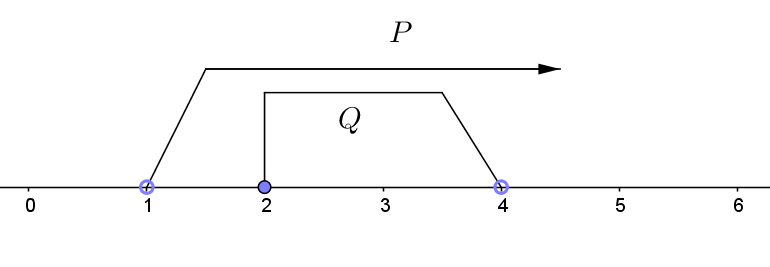
\includegraphics[width=0.6\textwidth]{number_line}

\(P\not\subset Q\)이므로 명제 \(p\to q\)는 거짓이다.

이때 반례는 \(x>1\)은 만족하면서 \(2\le x<4\)는 만족하지 않는 원소들로, \(\frac32\), \(5\), \(6\) 등이다.
\end{enumerate}
\end{mdframed}

%
\prob{}
다음 명제의 참, 거짓을 판별하여라.
\begin{enumerate}
\item
\(x-2=0\)이면 \(x^2+x-6=0\)이다.
\item
\(x\)가 소수이면 \(x\)는 홀수이다.
\item
\(\triangle ABC\)가 정삼각형이면 \(\triangle ABC\)는 이등변삼각형이다.
\item
\(x\)가 무리수이면 \(x^2\)은 유리수이다.
\end{enumerate}

%%
\section{`모든'과 `어떤'이 들어있는 명제}

%
\exam{}
전체집합이 \(U=\{-2,-1,0,1,2\}\)일 때,
\setcounter{equation}{0}
\begin{gather}
`\text{모든 }x\text{에 대하여 }x^2+1>0\text{이다.'}\\
`\text{모든 }x\text{에 대하여 }x+1>0\text{이다.'}
\end{gather}
에서 (1)은 전체집합 \(U\)의 모든 원소에 대하여 \(x^2+1>0\)이므로 참이지만, (2)는 \(x=-2\)이거나 \(x=-1\)일 때 성립하지 않으므로 거짓이다.
조건 \(p\), \(q\)를 각각 \(p:x^2+1>0\), \(q:x+1>0\)이라고 하면 진리집합 \(P\), \(Q\)는 각각 \(P=U\), \(Q=\{0,1,2\}\neq U\)이다.

또 
\begin{gather}
`\text{어떤 }x\text{에 대하여 }x+1<0\text{이다.'}\\
`\text{어떤 }x\text{에 대하여 }x^2+1<0\text{이다.'}
\end{gather}
에서 (3)은 \(x=-2\)일때 성립하므로 참이지만, (4)는 \(x^2+1<0\)을 참으로 만드는 \(x\)값이 없으므로 거짓이다.
조건 \(r\), \(s\)를 각각 \(r:x+1<0\), \(s:x^2+1<0\)이라고 하면 진리집합 \(R\), \(S\)는 각각 \(R\neq\varnothing\), \(S=\varnothing\)이다.

\begin{mdframed}
%
\theo{`모든'과 `어떤'이 포함된 명제의 참, 거짓}
전체집합을 \(U\), 조건 \(p\)의 진리집합을 \(P\)라고 하면
\begin{enumerate}
\item
`모든 \(x\)에 대하여 \(p\)이다.'는\\
\(P=U\)이면 참이고, \(P\neq U\)이면 거짓이다.
\item
`어떤 \(x\)에 대하여 \(p\)이다.'는\\
\(P\neq\varnothing\)이면 참이고, \(P=\varnothing\)이면 거짓이다.
\end{enumerate}
\end{mdframed}

\clearpage
%
\exam{}
\begin{enumerate}
\item
명제 `모든 실수 \(x\)에 대하여 \(x^2\ge0\)이다'는 \(\{x\ba x^2\ge0\}=U\)이므로 참이다.
\item
명제 `어떤 실수 \(x\)에 대하여 \(x^2<0\)이다'는 \(\{x\ba x^2<0\}=\varnothing\)이므로 거짓이다.
\end{enumerate}

%
\prob{}
다음 명제의 참, 거짓을 판별하여라.
\begin{enumerate}
\item
어떤 실수 \(x\)에 대하여 \(x^2=2x\)이다.
\item
\(x<1\)인 모든 실수 \(x\)에 대하여 \(x^2<1\)이다.
\end{enumerate}

\clearpage
%
\exam{}
세 학생 \(a\), \(b\), \(c\)에 대하여, 다음 네 명제를 생각해보자.
\setcounter{equation}{0}
\begin{gather}
\text{모든 학생은 남자이다.}\\
\text{모든 학생은 여자이다.}\\
\text{어떤 학생은 남자이다.}\\
\text{어떤 학생은 여자이다.}
\end{gather}

\kswrapfig[Pos=r]{allsome}{
명제 (1)의 부정이 무엇인지 한번 생각해보자.
`모든 학생은 남자이다'의 부정이니 `모든 학생은 여자이다'라고 답하기 쉽지만 실제로 그렇지 않다.

세 학생의 성별의 가능한 경우를 모두 나열해보면 오른쪽 그림과 같은데, 명제 (1)이 성립하는 경우의 반대는 명제 (4)이다.
따라서 명제 (1)의 부정은 (4)이다.
즉
\begin{center}
\fbox{모든 학생은 남자이다.}
\end{center}
의 부정은
\begin{center}
\fbox{어떤 학생은 남자가 아니다.}
\end{center}
이다.
}

\begin{mdframed}
%
\theo{`모든'과 `어떤'이 포함된 명제의 부정}
\begin{enumerate}
\item
명제 `모든 \(x\)에 대하여 \(p\)이다.'의 부정은
\begin{center}
`어떤 \(x\)에 대하여 \(\sim p\)이다.'
\end{center}
\item
명제 `어떤 \(x\)에 대하여 \(p\)이다.'의 부정은
\begin{center}
`모든 \(x\)에 대하여 \(\sim p\)이다.'
\end{center}
\end{enumerate}
\end{mdframed}

\clearpage
%
\exam{}
명제 `모든 실수 \(x\)에 대하여 \(x^2\ge1\)이다'의 부정을 말하고, 그것의 참, 거짓을 판별하여라.
\begin{mdframed}
주어진 명제의 부정은 `어떤 실수 \(x\)에 대하여 \(x^2<1\)이다'가 된다.
\(x^2<1\)의 진리집합은 \(\{x\ba x^2<1\}=\{x\ba-1<x<1\}\neq\varnothing\)이므로 주어진 명제의 부정은 참이다.
\end{mdframed}

%
\prob{}
주어진 명제의 부정을 말하고, 그것의 참, 거짓을 판별하여라.
\begin{enumerate}
\item
모든 정사각형은 마름모이다.
\item
어떤 정수는 자연수이다.
\item
모든 실수 \(x\)에 대하여 \(|x-1|>0\)이다.
\item
어떤 실수 \(x\)에 대하여 \(x^2=x\)이다.
\end{enumerate}

%%
\section*{확인문제}
%
\prob{}
다음 중 명제인 것을 찾고, 그것의 참, 거짓을 판별하여라.
\begin{enumerate}
\item
\(x^2-3x+2=0\)
\item
\(6\)의 약수는 \(12\)의 약수이다.
\end{enumerate}

%
\prob{}
두 조건 \(p\), \(q\)가 다음과 같을 때, 명제 \(p\to q\)의 참, 거짓을 판별하여라.
\begin{enumerate}
\item
\(p:x>2\),	\tabto{0.5\textwidth}\(q:x^2-1>0\)
\item
\(p:x^2-4=0\),	\tabto{0.5\textwidth}\(q:x-2=0\)
\end{enumerate}

%
\prob{}
다음 명제의 참, 거짓을 판별하여라.
또 거짓인 것은 반례를 들어라.
\begin{enumerate}
\item
모든 소수는 홀수이다.
\item
전체집합 \(U=\{1,2,5,10\}\)에 대하여 어떤 \(x\)는 짝수이다.
\end{enumerate}

%%
\section*{답}

%
\an{3}
\vspace{-20pt}
\begin{enumerate}
\item
명제이다, 참.
\item
명제이다, 거짓.
\item
명제가 아니다.
\item
명제가 아니다.
\end{enumerate}

%
\an{6}
\vspace{-20pt}
\begin{enumerate}
\item
가정 : \(x=2\)이다., 결론 : \(2x+3=7\)이다.
\item
가정 : 두 수 \(a\), \(b\)가 짝수이다, 결론 : \(a+b\)가 짝수이다.
\item
가정 : 두 삼각형이 서로 닮음이다., 결론 : 두 삼각형의 넓이가 서로 같다.
\end{enumerate}

%
\an{8}
\vspace{-20pt}
\begin{enumerate}
\item
두 변의 길이가 같은 삼각형
\item
평면 위의 한 점으로부터의 거리가 일정한 모든 점들의 집합
\item
한 각이 직각인 삼각형
\item
마주보는 한 쌍의 변이 서로 평행이 사각형
\end{enumerate}

%
\an{10}
정리, \(\overline{PA}=\overline{PB}\)이다., 증명

%
\an{13}
(1)\:\:
\(\{2,4,6\}\)
\tabto{0.5\textwidth} (2)\:\:
\(\{1,5\}\)
\par\noindent (3)\:\:
\(\{2,3,4,5,6\}\)
\tabto{0.5\textwidth} (4)\:\:
\(\{1,2,4\}\)

%
\an{17}
(1)\:\:
\(6\)은 합성수가 아니다.
\tabto{0.5\textwidth} (2)\:\:
\(0\notin\varnothing\)
\par\noindent (3)\:\:
\(x\)는 3의 배수가 아니다.
\tabto{0.5\textwidth} (4)\:\:
\(x-1<0\)

%
\an{19}
(1)\:\:
\(x\)는 홀수가 아니다, \(\{2,4,6\}\)
\tabto{0.5\textwidth} (2)\:\:
\(x<3\), \(\{1,2\}\)
\par\noindent (3)\:\:
\((x-1)(x-4)\neq0\), \(\{2,3,5,6\}\)
\tabto{0.5\textwidth} (4)\:\:
\(x^2>4\), \(\{3,4,5,6\}\)

%
\an{24}
(1)\:\:
참
\tabto{0.5\textwidth} (2)\:\:
거짓
\par\noindent (3)\:\:
참
\tabto{0.5\textwidth} (4)\:\:
거짓

%
\an{28}
(1)\:\:
참
\tabto{0.5\textwidth} (2)\:\:
거짓

%
\an{32}
\begin{enumerate}
\item
`어떤 정사각형은 마름모가 아니다.', 거짓
\item
`모든 정수는 자연수가 아니다.', 거짓
\item
`어떤 실수 \(x\)에 대하여 \(|x-1|\le0\)이다.', 참
\item
`모든 실수 \(x\)에 대하여 \(x^2\neq x\)이다.', 거짓
\end{enumerate}

%
\an{33}
(1)\:\:
명제가 아니다.
\tabto{0.5\textwidth} (2)\:\:
명제이다, 참

%
\an{34}
(1)\:\:
참
\tabto{0.5\textwidth} (2)\:\:
거짓

%
\an{35}
(1)\:\:
거짓, 반례는 2
\tabto{0.5\textwidth} (2)\:\:
참

\end{document}